\documentclass{book}
\usepackage{graphicx}
\usepackage{gb4e}
\usepackage{tipa}
\usepackage{natbib}
\usepackage[utf8]{inputenc}

\graphicspath{ {../images/} }

\newcommand{\entry}[4]{\textbf{#1} -- /\textipa{#2}/ \emph{#3} $\bullet$ #4\\}

\begin{document}

\begingroup
\centering
\vfill
\Huge{REFERENCE \\ GRAMMAR}\\
\huge{\&}\\
\Huge{DICTIONARY}\\
\huge{of}\\
\Huge{Sutlun}\\
\vspace{1cm}
\large{By Samuel Pearce}\\
\vfill\null
\endgroup
\thispagestyle{empty}

\tableofcontents
\pagebreak




\part{Grammar}
\chapter{Phonology}
\section{Consonants}
\begin{center}
    \begin{tabular}{l|c|c|c}
                    & Bilabial          & Alveoalar  & Palatal \\
        \hline
        Nasal       & m                 & n         &  \\
        Plosive     & p                 & t         & k \\
        Fricative   & \textipa{F} [f]   & s         & x \\
        Liquid      & w                 & l         & j \\
    \end{tabular}
\end{center}


\section{Vowels}
\begin{center}
    \begin{tabular}{l|c|c|c}
                    & Front                         & Back \\
        \hline
        Close       & i $\cdot$ y                   & \textipa{W [2]} $\cdot$ u \\
        Middle      & e                             & \\
        Open        & \textipa{a} [\ae] $\cdot$ \oe & \\
    \end{tabular}
\end{center}


\section{Phonotactics}
In Sutlun, roots are bi-consonantal and the vowel determines what part of speech the word is.
For these root words, the consonant structure is \textbf{CVC} Where V is any vowel except /\textipa{@}/
and C is any consonant. The root word is also always stressed. This applies for compounds as well:

\begin{center}
    ``jupympul'' $\rightarrow$ \textipa{/ju.pim."pul/} $\rightarrow$ ``Heavy rain''
\end{center}

Roots are the core of lexicon, there are only a handful of words which are not roots. These include:
\begin{itemize}
    \item `ek' \& `ke' are typically used as prefixes to form the negative form and the binary question
    form of words, but when used alone they stand for `no' \& `yes', respectively.
    \item `uwu' acts as the conditional marker, it's placed at the end of a sentence to indicate that
    the next sentence is only true if the first one is.
    \item `awa' acts as the negative conditional marker, like `but' in English.
    \item `en' is a stand-in for the next clause. It allows relative clauses by
    essentially saying `this:'. It is treated like a noun and can have the same
    suffixes applied to it.
\end{itemize}

Here are some examples to clarify the meaning of the ``grammatical words''

\begin{exe}
    \ex
    \gll Ut ketyf puxe? ek.\\
    2S.NOM QUE.like food.ACC? no \\
    \glt ``Do you want some food? No.''
\end{exe}

\begin{exe}
    \ex
    \gll Pampul pym uwu, up fatsyn.\\
    down-water.NOM fall COND, 1S.NOM bad-feel. \\
    \glt ``If it rains, I'll be sad.''
\end{exe}

\begin{exe}
    \ex
    \gll Up tyf ene, úp kin wukfusem.\\
    1S.NOM like this.ACC, 1P.NOM go plant-place.DAT. \\
    \glt ``I like it when we walk in the park.''
\end{exe}


\section{Orthography}
\subsection{Romanisation}
The romanisation used might seem quite strange to an outside observer, but it was designed to
emphasize the duality of the main vowels (y, ú, a) with their rounded equivalents (ý, u, á) which
represents a change in meaning for the roots. Please note that the unrounded 'u' is marked, whereas
the other two unrounded main vowels aren't, this is due to front vowels typically being unrounded,
while back vowels are typically rounded \cite{Stevens72}. The more ``typical'' vowel is the ``default'' form,
while the less typical form is the inflected one. Though given that this might be difficult to understand
and not as easy to type as it is on a QWERTZ keyboard, a more phonetic alternative is also provided with
digraph alternatives to the diacritics used.

\begin{center}
    \begin{tabular}{|c|c|c|}
        \hline
        IPA & Rom. & Alt. \\
        \hline
        p           & p & p \\
        t           & t & t \\
        k           & k & k \\
        m           & m & m \\
        n           & n & n \\
        \textipa{F} & f & f \\
        s           & s & s \\
        x           & x & x \\
        \textipa{@} & e & e \\
        \hline
    \end{tabular}
    \begin{tabular}{|c|c|c|}
        \hline
        IPA & Rom. & Alt. \\
        \hline
        w           & w & w \\
        l           & l & l \\
        j           & j & j \\
        a           & a & a \\
        \oe         & á & ö/oe \\
        i           & y & i \\
        y           & ý & ü/ue \\
        \textipa{W} & ú & ue \\
        u           & u & uu/oo \\
        \hline
    \end{tabular}
\end{center}

\subsection{Writing System}
Given the rigidly structured syllables, I experimented with the idea of writing systems that used this
to their advantage for more regular and compact glyphs, but found this too complicated and received
feedback that confirmed this fear. So I decided to go for a simpler alphabetic system for the writing
system. I definitely wanted to make it a featural system though, because I had layed the phonemes out
in a systematic manner for this purpose.

\begin{figure}
	\centering
	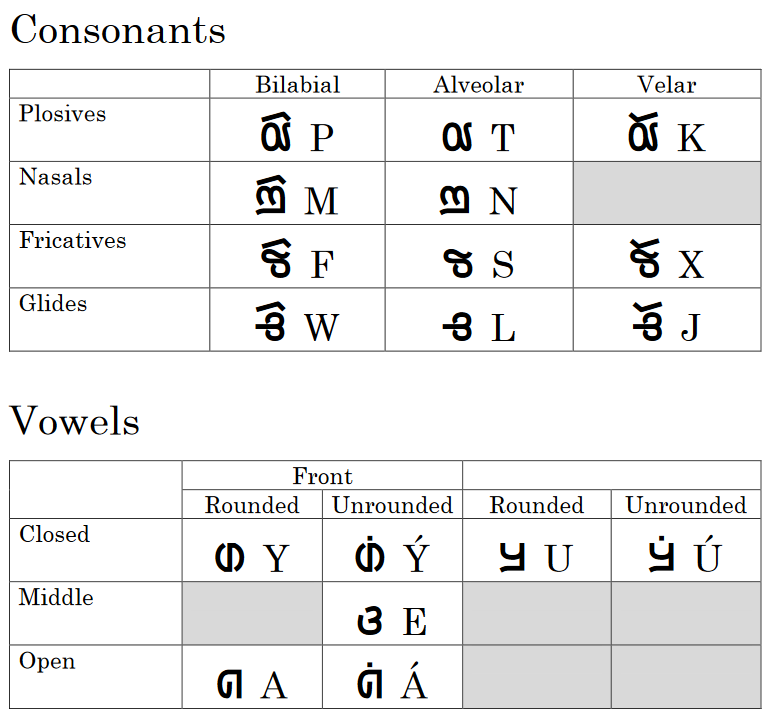
\includegraphics[scale=0.5]{Lumlun-Diagram.png}
	\caption{A diagram of all the letters in Lumlun, the writing system for Sutlun}
	\label{lumlun-diagram}
\end{figure}



\chapter{Morphology}
\section{Universal Inflections}
These are a few inflections (mostly prefixes) which can be applied to any root, no matter the
part of speech. Though these changes may not always yield a result that fully makes sense.

\subsection{Opposites}
You can form the opposite meaning of a word by flipping the root's consonants:

\begin{center}
    ``taf'' $\rightarrow$ ``good'' \\
    ``fat'' $\rightarrow$ ``bad''
\end{center}

\subsection{Negation}
To negate anything, simply prefix it with ``ek-''. For nouns, this forms the phrase ``not X'', where X
is the negated noun e.g.

\begin{center}
    ``pux'' $\rightarrow$ ``food'' \\
    ``ekpux'' $\rightarrow$ ``not food''
\end{center}

For Verbs, this means to not do the action:

\begin{center}
    ``pýx'' $\rightarrow$ ``eat'' \\
    ``ekpýx'' $\rightarrow$ ``don't eat''
\end{center}

And for adjectives, it means not like the adjective:

\begin{center}
    ``pax'' $\rightarrow$ ``delicious'' \\
    ``ekpax'' $\rightarrow$ ``not delicious''
\end{center}

It is important to bear in mind the difference between negation and opposites, as they often
seem to share the same meaning, but ``not good'' is not the same as ``bad''.

\subsection{Binary Question Prefix}
If you wish to ask a binary (yes or no) question, you can simply add the `ke-' prefix to the
verb, or to any word you wish to emphasize. E.g.:

\begin{exe}
    \ex
    \gll Ut ketyf múne?\\
    2S.NOM QUE-like game.P.ACC? \\
    \glt ``Do you like games?''
\end{exe}


\section{Nouns}
\subsection{Number}
In Sutlun, Nouns all have the ``u'' sound in the root which is unrounded for singular and rounded for plural.
For example:

\begin{center}
    ``mun'' $\rightarrow$ ``a game'' \\
    ``mún'' $\rightarrow$ ``many games''
\end{center}

\subsection{Case}
Sutlun has 4 grammatical cases which are all formed with a simple suffix according to the following table:

\begin{center}
    \begin{tabular}{|r|l|l|}
        \hline
        Case Name   & Suffix    & Example \\
        \hline
        Nominative  & -         & pux \\
        Accusative  & -e        & puxe \\
        Dative      & -em       & puxem \\
        Genitive    & -es       & puxes \\
        \hline
    \end{tabular}
\end{center}

\subsection{Definitiveness}
By default, nouns are indefinite and if they are definite, it can be parsed through context,
but if you wish to define a noun as being definite, you can give it the `-te' prefix.

\begin{center}
    ``mun'' $\rightarrow$ ``a game'' \\
    ``temun'' $\rightarrow$ ``the game''
\end{center}


\section{Verbs}
\subsection{Mood}
Sutlun has two verb moods: Indicative \& Imperative. These are also formed by the root-sound's roundness.
All Verbs use the ``y'' sound for their roots. ``Y'' is indicative, while ``ý'' is imperative:

\begin{center}
    ``ut kyn'' $\rightarrow$ ``You go.'' / ``You are going.'' \\
    ``ut kýn'' $\rightarrow$ ``You, go!''
\end{center}

\subsection{Tense}
Sutlun has 3 tenses which are all formed with a simple suffix according to the following table:

\begin{center}
    \begin{tabular}{|r|l|r|l|}
        \hline
        Tense Name  & Suffix    & Example   & Meaning \\
        \hline
        Past        & -et       & pixet     & ate, were eating \\
        Present     & - (-ef)   & pix       & eat, are eating \\
        Future      & -ej       & pixej     & will eat \\
        \hline
    \end{tabular}
\end{center}
The present tense is the default tense and needn't be marked, but if it is, it emphasizes that
the action is taking place now. E.g.:

\begin{center}
    ``ut kyn kumem?'' $\rightarrow$ ``Where are you going?'' \\
    ``ut kynef kumem?'' $\rightarrow$ ``Where are you going now?''
\end{center}


\section{Adjectives}
\subsection{Positive \& Superlative}
Adjectives in Sutlun all have the ``a'' sound in their root which is rounded to form the superlative
form of the adjective.

\begin{center}
    ``taf pux'' $\rightarrow$ ``good food'' \\
    ``táf pux'' $\rightarrow$ ``the best food''
\end{center}

Adjectives may also be used alone in the position of the verb of the sentence to mean ``to be like X''. i.e.:

\begin{center}
    ``ut taf'' $\rightarrow$ ``You're good.'' \\
    ``mukmun mán'' $\rightarrow$ ``This game is the most fun.''
\end{center}

\subsection{Comparing}
To form the comparative of an adjective, you add the augmentative or diminutive prefix, depending
on whether you want the positive or negative form:

\begin{center}
    ``upes xul jutaf.'' $\rightarrow$ ``My house is better.'' \\
    ``ukes puxe ujtaf utes puxem'' $\rightarrow$ ``Their food is worse than your food.'' \\
    ``ut kenik juwas mun?'' $\rightarrow$ ``Did you get a newer game?''
\end{center}


\section{Other}
Some roots also allow a fourth option using `e' as the vowel. This changes meaning from word to word
and is really the only exception, but it is possible to use the language without the ``e-words''.

For some words the ``e-form'' is a preposition for when the implied preposition is not clear, or when
it needs to be overridden. e.g.:

\begin{exe}
    \ex
    \gll Up puxe kin nek úkem.\\
    1S.NOM food.ACC from.PREP 3P.DAT. \\
    \glt ``I bring food from them.''
\end{exe}

For other words, this is more of an expletive, for example ``kem'' which acts a general exclamation
of surprise, i.e. ``What!?''

Some e-words are conjugations, such as ``xel'' which I've interpreted to mean ``and''.
E.g.: ``Up xel ut'' $\rightarrow$ ``You and I''.

The meaning of these words is fairly flexible though and can be left to interpretation. If I've seen
a useful possible meaning, though, I have noted it in the dictionary at the end of this grammar.



\chapter{Syntax}
\section{Phrases}
All forms of phrase follow the same order for dependents:

\begin{center}
    Preposition/Demonstrative $\rightarrow$ Posessor $\rightarrow$ Adjectives (No internal order) $\rightarrow$ HEAD
\end{center}

An example of all of these together would be:

\begin{center}
    ``xel upes taf jumuklumxul'' $\rightarrow$ ``In my good, big house.''
\end{center}

\section{Compounds}
Compounds can be formed from any type of speech with only the last determining what
the whole compound is. E.g.: ``jupympul'' $\rightarrow$ ``big falling water'' $\rightarrow$ ``heavy rain''.

At the core of the compund is the grouping of roots with no suffixes or prefixes. Then suffixes and
preixes may be added on to the compound as a whole.


\section{Sentence Order}
The most common order for a sentence is SVO in Sutlun, but because it has case marking, the
order is almost completely free:

\begin{exe}
    \ex
    \gll ukes lumxulem up kin puxe \\
    3S-GEN house-DAT 1S-NOM move-to food-ACC \\
    \glt ``I take food to his house.''
\end{exe}

The only exception is that a genitive must always be placed immediately before its posessum, unless there
is only one noun in the sentence:

\begin{center}
    \begin{exe}
        \ex ukes lumxulem up ...
        \ex[*] {lumxulem up ukes ...}
    \end{exe}
\end{center}


\section{Conditionals}
Conditionals, as have been mentioned previously are quite simple:
To indicate that a clause is predicated on a previous clause, you
can join them with ``uwu,'':

\begin{exe}
    \ex
    \gll Pampul pym uwu, up fatsyn.\\
    down-water.NOM fall COND, 1S.NOM bad-feel. \\
    \glt ``If it rains, I'll be sad.''
\end{exe}


\section{Subordinate Clauses}
As also previously mentioned, subordinate clauses are created by
using ``en'' as a stand-in noun representing the succeeding clause:

\begin{exe}
    \ex
    \gll Up tyf ene, úp kin wukfusem.\\
    1S.NOM like this.ACC, 1P.NOM go plant-place.DAT. \\
    \glt ``I like it when we walk in the park.''
\end{exe}

`En' can also be used to mean the previous sentence or statement, generally when it's 
used at the beginning of a sentence. The author/speaker should make it clear which is
meant through context.

If no `en' or other conjunction is used in the sentence before a clause,
it counts as being grouped with the previous phrase.
E.g.:

\begin{exe}
    \ex
    \gll Úk sutlynet ene úkem, úk týlej wamlume, úk jufýlej wamlume.\\
    1P.NOM air-word.PST this.ACC 1P.DAT, 1P.NOM make.IMP.FUT flat-stone.ACC, 1P.NOM AUG.heat.IMP.FUT flat-stone.ACC. \\
    \glt ``We said to ourselves: `we shall make bricks and we shall fire the bricks well.'''
\end{exe}



\part{Lexicon}

\begin{center}
    \Huge{P}
\end{center}

{\Large\textbf{P-X} -- Food, Drink} \\
\emph{Antonym: ``Excretion, Expelling'' See X-P} \\
\entry{pux}{"pux}{n. sg.}{Food, Drink, an item of food, a meal}
\entry{púx}{"p2x}{n. pl.}{Food, many items of food/drink}
\entry{pyx}{"pix}{v. ind.}{to eat, to drink, to consume}
\entry{pýx}{"pyx}{v. imp.}{eat!, drink!, consume!}
\entry{pax}{"pax}{a. pos.}{delicious, tasty}
\entry{páx}{"p\oe x}{a. sup.}{most delicious}

\begin{center}
    \Huge{T}
\end{center}

{\Large\textbf{T-F} -- Good, Positive} \\
\emph{Antonym: ``Bad, Negative'' See F-T} \\
\entry{tuf}{"tuf}{n. sg.}{a good deed/thing, the concept of goodness}
\entry{túf}{"t2f}{n. pl.}{many good things}
\entry{tyf}{"tif}{v. ind.}{to improve, fix, better}
\entry{týf}{"tyf}{v. imp.}{fix!, improve!}
\entry{taf}{"taf}{a. pos.}{good, well}
\entry{táf}{"t\oe f}{a. sup.}{the best}

{\Large\textbf{T-S} -- Quiet, Still} \\
\emph{Antonym: ``Noise, Sound, Loud'' See S-T} \\
\entry{tus}{"tus}{n. sg.}{quiet, peace, stillness}
\entry{tús}{"t2s}{n. pl.}{much stillness, much peace}
\entry{tys}{"tis}{v. ind.}{to be quiet, calm down, make peace}
\entry{týs}{"tys}{v. imp.}{be quiet!, calm down!}
\entry{tas}{"tas}{a. pos.}{good, well}
\entry{tás}{"t\oe s}{a. sup.}{the best}

\begin{center}
    \Huge{K}
\end{center}

{\Large\textbf{K-M} -- Query, What?} \\
\emph{Antonym: ``Demonstrative, Thing, That'' See M-K} \\
\entry{kum}{"kum}{n. sg.}{what thing?}
\entry{kúm}{"k2m}{n. pl.}{what things?}
\entry{kym}{"kim}{v. ind.}{doing what?}
\entry{kým}{"kym}{v. imp.}{(special case) what are you doing?}
\entry{kam}{"kam}{a. pos.}{like what?}
\entry{kám}{"k\oe m}{a. sup.}{most like what?}
\entry{kem}{"kem}{excl.}{What!? (General indicator of confusion)}

{\Large\textbf{K-N} -- Go, Move, Give} \\
\emph{Antonym: ``Come, Bring'' See N-K} \\
\entry{kun}{"kun}{n. sg.}{a walk, a motion/movement, a journey}
\entry{kún}{"k2n}{n. pl.}{many walks, many motions/movements, many journeys}
\entry{kyn}{"kin}{v. ind.}{to walk, to move, to go}
\entry{kýn}{"kyn}{v. imp.}{walk!, move!, go!}
\entry{kan}{"kan}{a. pos.}{in motion, moving, going, living}
\entry{kán}{"k\oe n}{a. sup.}{moving the most, the most alive}
\entry{ken}{"ken}{prep.}{to, toward}

{\Large\textbf{K-F} -- Fantasy, Unreal, Fake} \\
\emph{Antonym: ``Thing, Real, Exist'' See F-K} \\
\entry{kuf}{"kuf}{n. sg.}{a fantasy, something fake/unreal}
\entry{kúf}{"k2f}{n. pl.}{many fantasies, unreal things}
\entry{kyf}{"kif}{v. ind.}{imagine, picture}
\entry{kýf}{"kyf}{v. imp.}{iamge!, picture!}
\entry{kaf}{"kaf}{a. pos.}{fake, unreal, fantasy, fictional}
\entry{káf}{"k\oe f}{a. sup.}{the most fake, unreal, fictional}

\begin{center}
    \Huge{M}
\end{center}

{\Large\textbf{M-K} -- Demonstrative, Thing} \\
\emph{Antonym: ``Query, What?'' See K-M} \\
\entry{muk}{"muk}{n. sg.}{this/that thing}
\entry{múk}{"m2k}{n. pl.}{these/those things}
\entry{myk}{"mik}{v. ind.}{doing this/that}
\entry{mýk}{"myk}{v. imp.}{do this/that!}
\entry{mak}{"mak}{a. pos.}{like this/that}
\entry{mák}{"m\oe k}{a. sup.}{most like this/that}

{\Large\textbf{M-N} -- Entertainment, Fun, Game} \\
\emph{Antonym: ``Work, Task, Boring'' See N-M} \\
\entry{mun}{"mun}{n. sg.}{a game, book, film, TV-show, play, etc.}
\entry{mún}{"m2n}{n. pl.}{many games, books, films, etc.}
\entry{myn}{"min}{v. ind.}{to play, entertain, relax}
\entry{mýn}{"myn}{v. imp.}{go play!, have fun!}
\entry{man}{"man}{a. pos.}{fun, entertaining}
\entry{mán}{"m\oe n}{a. sup.}{most fun, entertaining}

{\Large\textbf{M-L} -- Soft, Weak, Clay} \\
\emph{Antonym: ``Solid, Strong, Rock, Metal'' See L-M} \\
\entry{mul}{"mul}{n. sg.}{a soft thing, some clay, sand, paste, powder}
\entry{múl}{"m2l}{n. pl.}{many soft things, clay, sand, paste, powder}
\entry{myl}{"mil}{v. ind.}{to soften, weaken, mould}
\entry{mýl}{"myl}{v. imp.}{soften!, weaken!, mould!}
\entry{mal}{"mal}{a. pos.}{soft, weak}
\entry{mál}{"m\oe l}{a. sup.}{most soft, weak}

\begin{center}
    \Huge{N}
\end{center}

{\Large\textbf{N-M} -- Work, Task, Boring} \\
\emph{Antonym: ``Entertainment, Fun, Game'' See M-N} \\
\entry{num}{"num}{n. sg.}{a task, job, craft, skill}
\entry{núm}{"n2m}{n. pl.}{many tasks, jobs, crafts, skills}
\entry{nym}{"nim}{v. ind.}{to work, make, craft}
\entry{ným}{"nym}{v. imp.}{work!, maake!, craft!}
\entry{nam}{"nam}{a. pos.}{mandatory, boring, arduous}
\entry{nám}{"n\oe m}{a. sup.}{most boring, arduous}

{\Large\textbf{N-F} -- Like, Desire, Want} \\
\emph{Antonym: ``Dislike, Hate, Must'' See F-N} \\
\entry{nuf}{"nuf}{n. sg.}{a desire, want}
\entry{núf}{"n2f}{n. pl.}{many desires, wants}
\entry{nyf}{"nif}{v. ind.}{to like, desire, want}
\entry{nýf}{"nyf}{v. imp.}{like smth.! (special case:) exclamation of joy ``wow!'', ``yay!''}
\entry{naf}{"naf}{a. pos.}{nice , boring, arduous}
\entry{náf}{"n\oe f}{a. sup.}{most boring, arduous}

\begin{center}
    \Huge{F}
\end{center}

\begin{center}
    \Huge{S}
\end{center}

\begin{center}
    \Huge{X}
\end{center}

\begin{center}
    \Huge{W}
\end{center}

\begin{center}
    \Huge{L}
\end{center}

\begin{center}
    \Huge{J}
\end{center}

\begin{center}
    \Huge{I}
\end{center}

\begin{center}
    \Huge{U}
\end{center}

\begin{center}
    \Huge{A}
\end{center}

\begin{center}
    \Huge{E}
\end{center}

\bibliography{Bibliography}
\bibliographystyle{plain}

\end{document}
